\section{Auxilary Construction}\label{sec:auxiliaryConstruction}
Let $\Phi$ be a Boolean formula of P3SAT with variables $x_1,\ldots , x_n$ and clauses $C_1,\ldots ,C_m$, where $A(\Phi)$ is the associated planar graph and $\tilde{A}\lr{\Phi}$ be corresponding honeycomb graph.
We continue to modify $\tilde{A}\lr{\Phi}$ to form the auxilary construction.   
Consider a large (polynomial-size) regular hexagon $J$  with side length $s(n,m)$ that contains all gadgets in our construction and hexagonal grid.
For each hexagon of the hexagonal grid contained in $J$, scale the hexagon in the following way: first we fix the center of the hexagon and then scale (shrink) the hexagon; adjacent hexagons in the honeycomb no longer touch each other and form corridors and junctions between the hexagons (See Figure \ref{fig:ScalingForCorridors.pdf}). 

\begin{minipage}{\linewidth}
\begin{center}
\includegraphics[width=.4\columnwidth]{graphics/ScalingForCorridors.pdf}
\captionof{figure}{(a) This figure shows a region of a hexagonal grid scaled in place to form corridors between adjacent hexagons(shown in (b)).}\label{fig:ScalingForCorridors.pdf}
\end{center}
\end{minipage}

Formally, let a \textit{corridor} be a channel between two adjacent hexagons and a \textit{junction} be a region where three corridors meet.

\textbf{Formal Decscription of the Auxilary Construction.}
Given the side length of $J$, $s(n,m)$, we need to scale the grid of hexagons of the hexagonal grid in the interior of $J$ accordingly.

\begin{minipage}{\linewidth}
\begin{center}
\includegraphics[width=.9\columnwidth]{graphics/hexagonalConstructionOfJSmallWithoutHalfHexagons.pdf}
\captionof{figure}{(a) shows a \textit{formal auxilary construction} with $k=2$. $k$ is the number of hexagons of the hexagonal grid in the interior of $J$ that is on the bottom most row.  (b) shows a formal auxilary construction with $k=3$. (c) shows a formal auxilary construction with $k=4$.  Note that in each figure}\label{fig:hexagonalConstructionOfJSmallWithoutHalfHexagons.pdf}
\end{center}
\end{minipage}

In Figure \ref{fig:hexagonalConstructionOfJSmallWithoutHalfHexagons.pdf}, we show the three smallest possible formal constructions of $J$, $J_1, J_2, J_3$.  
A formal construction of $J$ is when six hexagons of the hexagonal grid each have two adjacent sides lie on the perimeter of $J$.
We have shown informal construction earlier where this does not occur.
Unless otherwise specified, we will assume the use formal constructions.
Each of the figures in Figure \ref{fig:hexagonalConstructionOfJSmallWithoutHalfHexagons.pdf} shows $J$ in bold and the hexagonal grid in its interior.
Notice that in each case we have six hexagons of the hexagonal grid with each of the six hexgaons having two adjacent sides that lie on the perimeter of $J$.

The height and diamater of $J$ can be described in terms of hexagons in the grid a vertical or horizontal line may cross. 
We'll denote these qualities as the hexagonal height and hexagonal diameter of $J$.  
Figures \ref{fig:hexagonalConstructionOfJSmallWithoutHalfHexagons.pdf}(c) and \ref{fig:hexagonalConstructionOfJSmallWithoutHalfHexagons.pdf}(a) show the hexagons of the hexagonal height and hexagonal diamters of $J_1$ and $J_3$ respectively.  
The formula for calculating hexagonal height of $J_z$ is 
\begin{equation}\label{eqn:Jh}
J_h (n,m) = 6z(n,m)+1
\end{equation}
The formula for calcuating the hexagonal diameter of $J_z$ is 
\begin{equation}\label{eqn:Jd}
J_d (n,m) = 4z(n,m)+1
\end{equation}
Since the associated graph of a P3SAT instance can be encoded into a honeycomb grid of size $s(n,m) \times s(n,m)$, then let $z(n,m)=4\cdot s(n,m)$ to enclose the same honeycomb to be enclosed into the interior of $J_z$.

% Figure \ref{fig:hexagonalConstructionOfJSmallWithoutHalfHexagons.pdf}(b) illustrates the side length of $J$ as $s(n,m)$ and half the height of $J$ as $s(n,m) \sqrt{3}$.
% For any $J$, there is a fixed number of hexagons in the hexagonal grid that lie on one side of the perimeter of $J$; denote this number as $k$.
% We can denote the number of hexagons in a row of the hexagonal grid in $J_z$ with the following sequence as follows:
% \begin{equation}\label{eqn:hexagonalGridSequence}
% \begin{array}{rcl}
% a(0) &=& k\\
% a(1) &=& k-1 \\
% a(2) &=& k\\
% a(i) &=& a(i-3)+1\\
% 0\leq&i&\leq \ceil{\frac{J_h (z)}{2}}
% \end{array}
% \end{equation}
% The $i^\text{th}$ number of Sequence \ref{eqn:hexagonalGridSequence} indicates the number of hexagons on the $i^\text{th}$ row of the hexagonal grid in the interior of $J$ from the perimeter of $J$ up to the half height of $J$. In Figure \ref{fig:hexagonalConstructionOfJSmallWithoutHalfHexagons.pdf}(c) from the bottom to the mid-height of $J$, the sequence $a(i)$ (i.e. the number of hexagons in each subsequent row) is 4, 3, 4, 5, 4, 5, 6, 5, 6, 7.
% Denote the hexagons of the hexagonal grid in $J$ as \textit{obstacle hexagons}.

\begin{minipage}{\linewidth}
\begin{center}
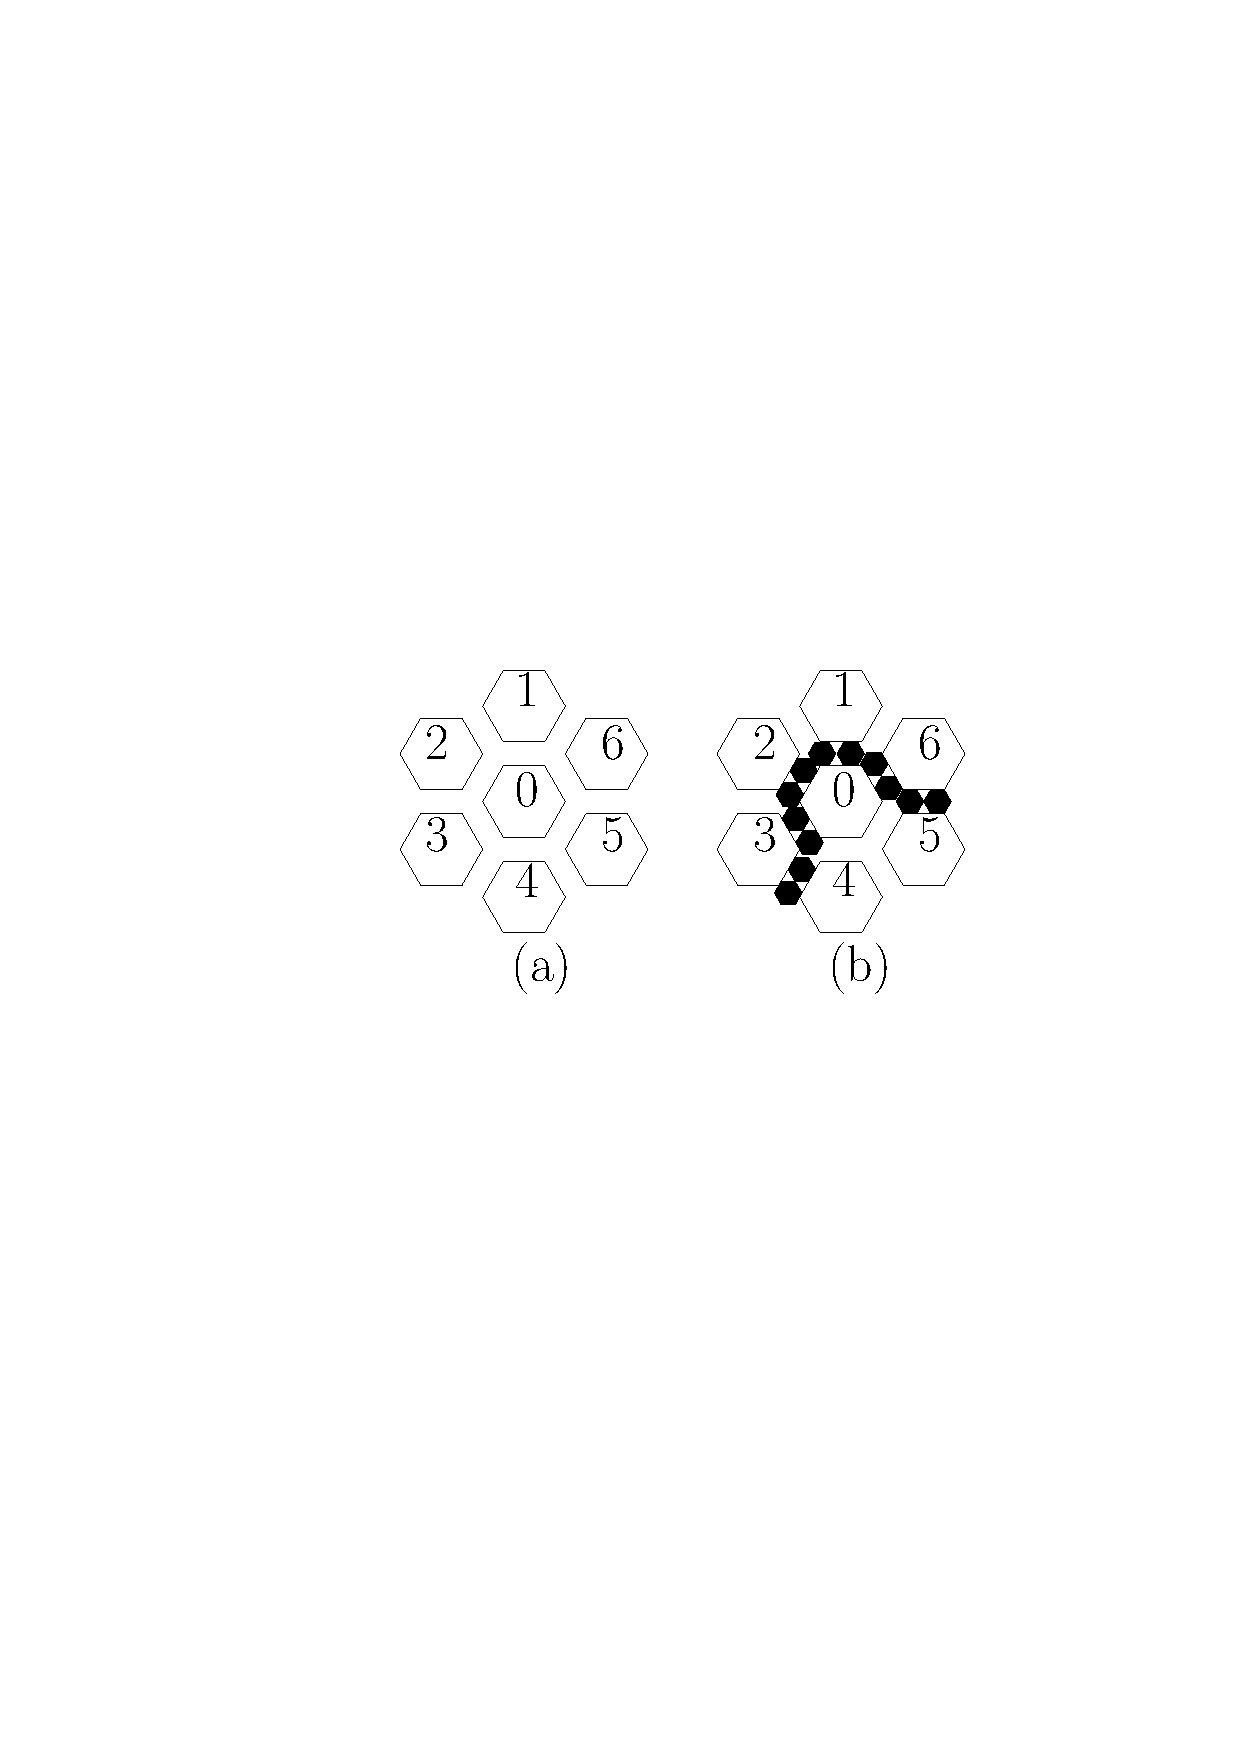
\includegraphics[scale=.66]{graphics/FlexibleHexagons.pdf}
\captionof{figure}{
(a) A region of the honeycomb shown with scaling. The corridors and junctions formed from the first scaling is preserved after scaling the honeycomb grid to where the side lengths of the hexagon are $N(n,m)$.
(b) The same region in (a) containing flags.
}\label{fig:HoneycombFlixible.pdf}
\end{center}
\end{minipage}

Let the numbered hexagons of Figure \ref{fig:HoneycombFlixible.pdf}(a) be obstacle hexagons that are fixed.
In Figure \ref{fig:HoneycombFlixible.pdf}(b), we have smaller hexagons within some corridors and junctions.
These hexagons are flags.
For each edge in $\tilde{A}(\Phi)$, we insert flags into the corridor corresponding to that edge.
Flags are hinged at the vertex closest to origin and the side of the corridor (See Figure \ref{fig:variable}).
Let $t(n,m)=s^\kappa$ be the number of flags in a corridor (see Figure \ref{fig:variable}). 
Scale $J$ and the obstacle hexagons in the interior of $J$ independently from their centers (see Figure \ref{fig:ScalingForCorridors.pdf}) such that each obstacle hexagon has side length: $$N(n,m)=\frac{5t(n,m)-1}{2}.$$ 

\begin{minipage}{\linewidth}
\begin{center}
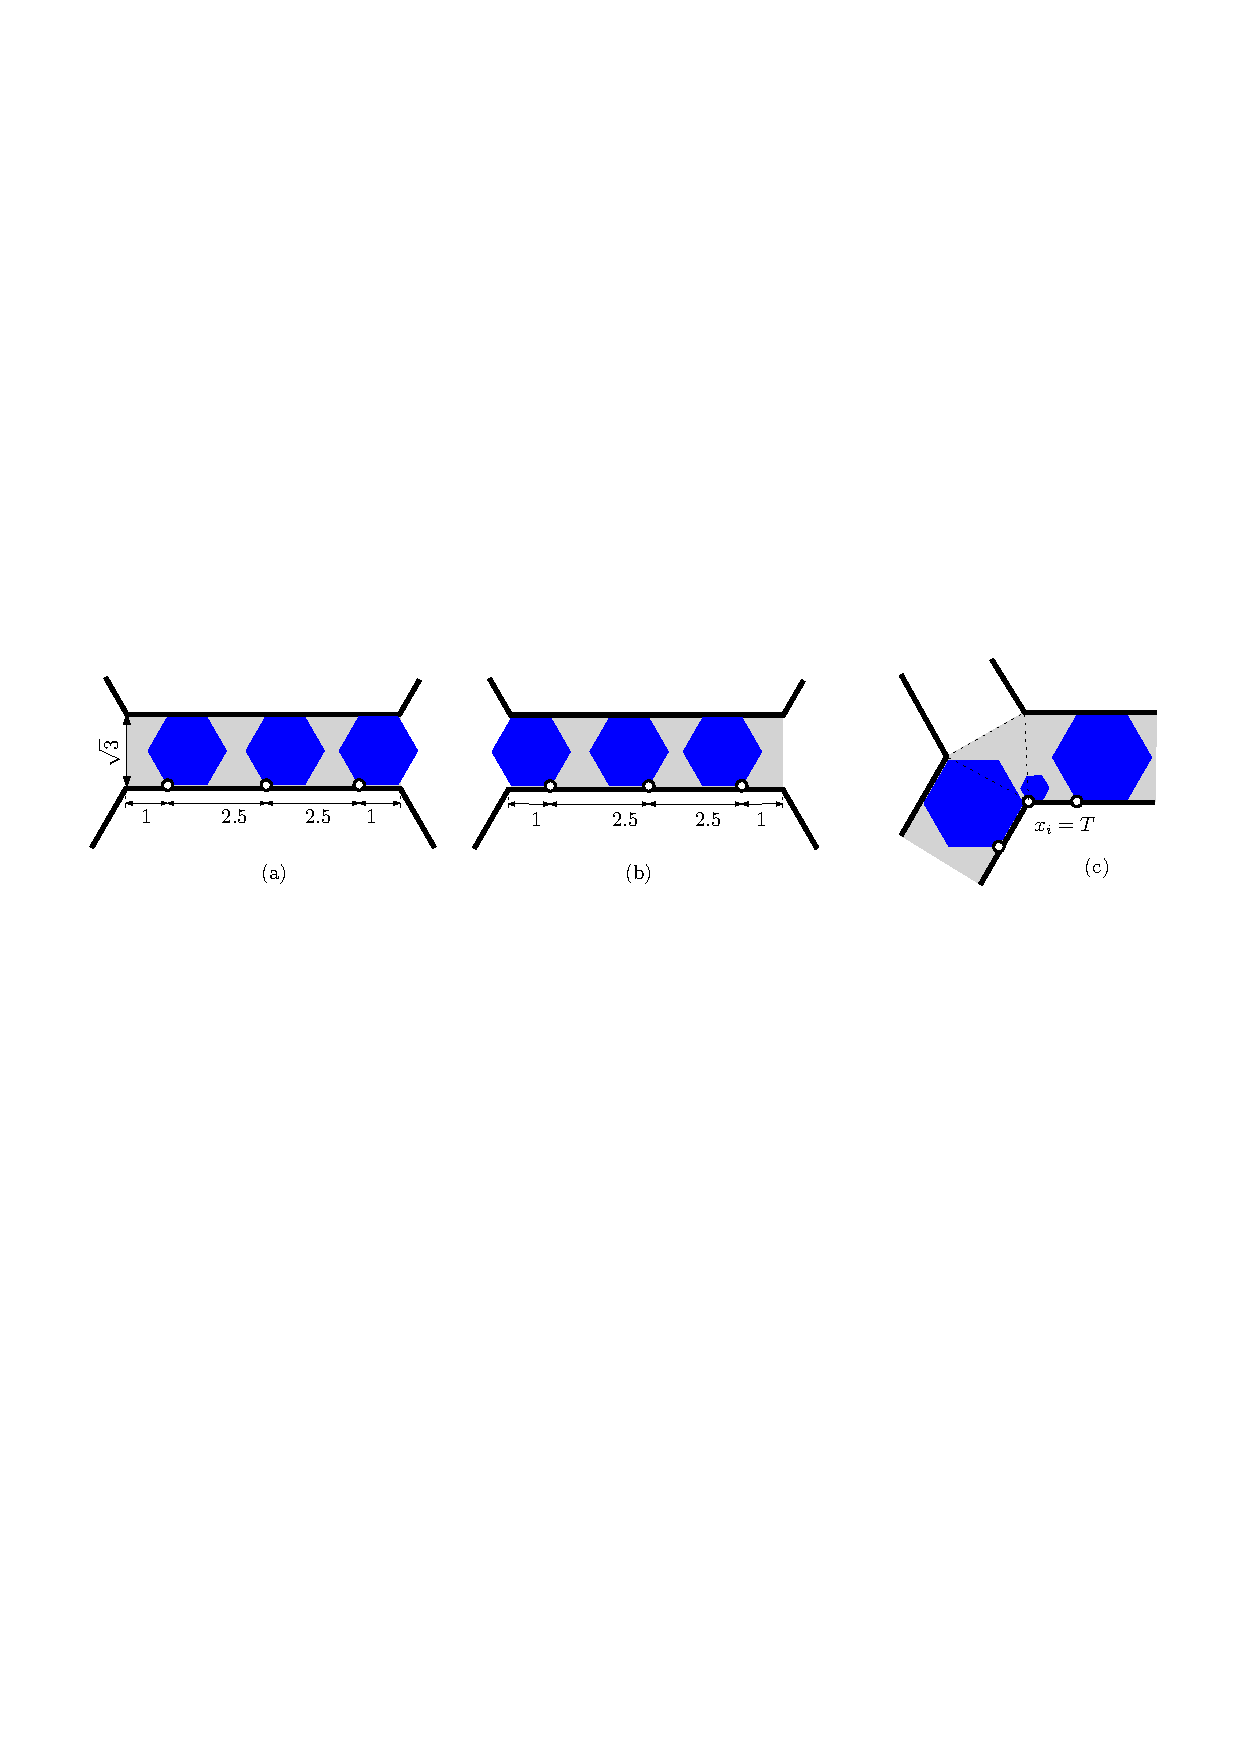
\includegraphics[width=0.9\columnwidth]{graphics/fig-variable-hex+}
\captionof{figure}{
(a) A corridor when all unit hexagons are in state R.
(b) A corridor where all unit hexagons are in state L.
(c) A junction where a small hexagon between two corridors
    ensures that at most one unit hexagon enters the junction from those corridors.}\label{fig:variable}
\end{center}
%\end{figure}
\end{minipage}

%These large hexagons are considered fixed obstacles in our auxiliary construction. 
Between two adjacent obstacle hexagons, there is a $\frac{5t-1}{2}\times \sqrt{3}$ rectanglar corridor.  %, which we call corridor. 
Three adjacent corridors meet at a regular triangle, which we call a junction. 

We next describe variable, clause, and transmitter gadgets.
The basic building block of both variable and transmitter gadgets consists of $t$ regular hexagons of side length 1 (\emph{unit hexagons}, for short) attached to a wall of a corridor such that the hinges divide the wall into $t+1$ intervals of length $(1,2.5,\ldots ,2.5,1)$ as shown in Fig.~\ref{fig:variable}(a-b). 

% In some of the junctions, we attach a small hexagon of side length $\frac{1}{3}$ to one or two corners of the junction (see Fig.~\ref{fig:variable}(c) and Fig.~\ref{fig:transmitter}). 

\paragraph{Variable Gadget.}
The {\bf variable gadget} for variable $x_i$ is constructed as follows. 
Recall that variable $x_i$ corresponds to a cycle in the associated graph $\tilde{A}(\Phi)$, which has been embedded as a cycle in the hexagonal tiling, with corridors and junctions. 
In each junction along this cycle, attach a small hexagon in the common boundary of the two corridors in the cycle. 
Figure \ref{fig:VariableGadgetSmall.pdf} depicts a \textit{variable gadget} in the hexagonal grid.

\begin{minipage}{\linewidth}
\begin{center}
\includegraphics[width=0.45\columnwidth]{graphics/VariableGadgetSmall.pdf}
\captionof{figure}{This depicts a variable gadget with $x_1 = T$.  Carefully note that the flags around $x_1$ are in the state $R$. Corridors adjacent to two obstacles of a variable in the honeycomb do not have $t$ flags; these corridors simply have the flags at the junctions.}\label{fig:VariableGadgetSmall.pdf}
\end{center}
\end{minipage}

For each junction in the transmitter gadget, we attach a small hexagon in the junction as shown in Figure \ref{fig:transmitter} except at the clause junction.
 A {\bf transmitter gadget} is constructed for each edge $\left\lbrace x_i,C_j\right\rbrace$ of the graph $A(\Phi)$; it consists of a sequence of junctions and corridors from a variable gadget's junction to a clause junction.  
Choosing the location of the small hexagon depends on whether the non-negated or negated literal is found in the clause.
\begin{itemize}
\item[(a)]  For an edge $(x_i,C_j)$ of the graph $A(\Phi)$, if the non-negated literal of $x_i$ exists in $C_j$, attach the small hexagon to the left side of the junction (see Figure \ref{fig:VariableJunctionTransmitterSelection.pdf}(a)).
\item[(b)]  For an edge $(x_i,C_j)$ of the graph $A(\Phi)$, if the negated literal of $x_i$ exists in $C_j$, attach thhe small hexagon to the right side of the junction (see Figure \ref{fig:VariableJunctionTransmitterSelection.pdf}(b)).
\end{itemize}
\paragraph{Clause Gadget.}
Recall that a clause from a Boolean formula $\Phi$ in 3-CNF has three literals.  If $\Phi$ is a  'yes' instance, then at least one literal in every clause of $\Phi$ is true.  We construct the clause gadget to model this fact about Boolean formulas in 3-CNF.

The {\bf clause gadget} lies at a junction adjacent to three transmitter gadgets (see Fig.~\ref{fig:clause} and Section \ref{transmitterGadget}). 
At such a junction, we attach a unit line segment to an arbitrary vertex of the junction, and a small hexagon of side length $\frac{1}{3}$ to the other end of the segment. 
If unit hexagons enter the junction from all three corridors (i.e., all three literals are false), then there is no space left for the small hexagon (see Lemma \ref{lem:aux-1}).

\begin{minipage}{\linewidth}
\begin{center}
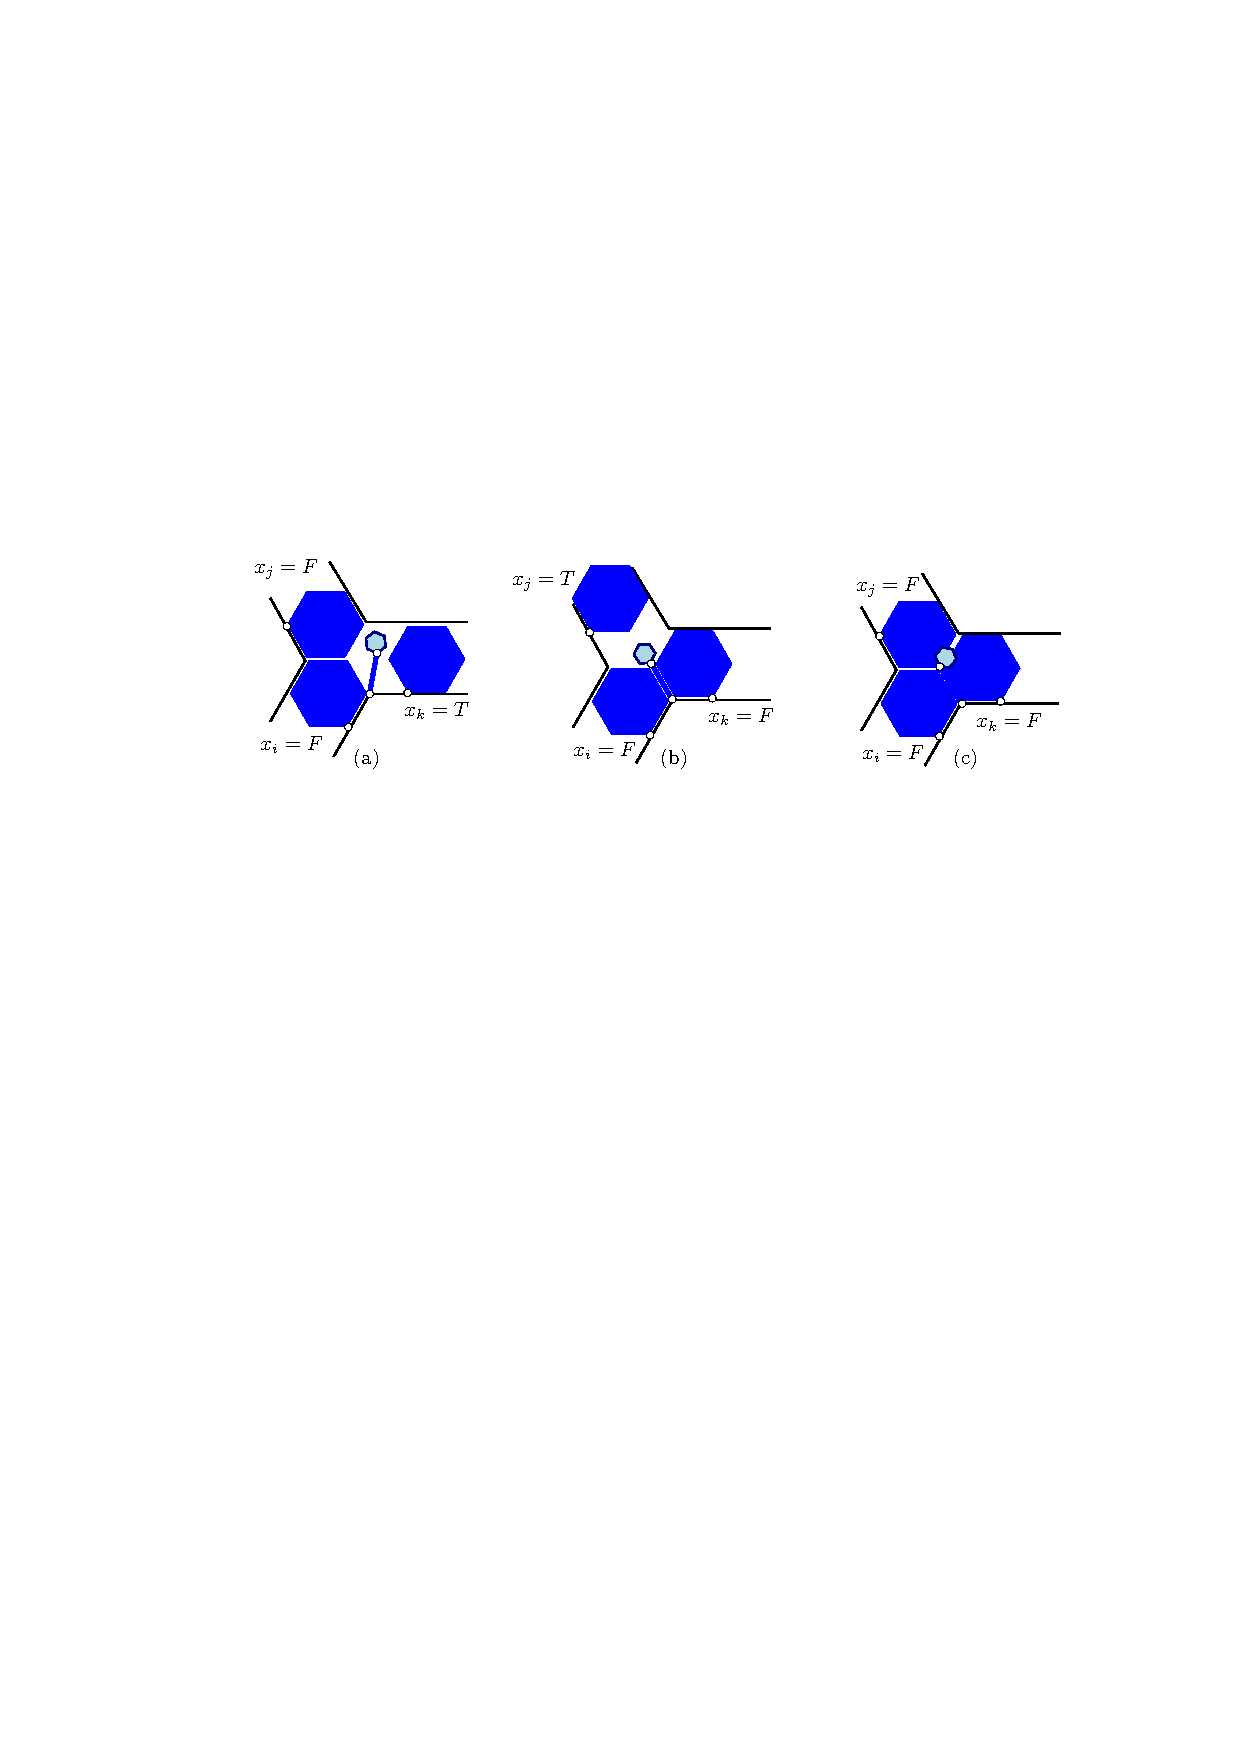
\includegraphics[width=0.7\columnwidth]{graphics/fig-clause-hex}
\captionof{figure}{(a-b) A clause gadget $(x_i\vee x_j\vee x_k)$ i\
    realizable when at least one of the literals is {\sc True}.
    (c) The clause gadget cannot be realized when all three literals are {\sc False}.}\label{fig:clause}
\end{center}
\end{minipage}

%But if at most two unit hexagons enter the junction (i.e., one of the literals is true), then the unit segment and the small hexagon are realizable.

\paragraph{Transmitter Gadget.}\label{transmitterGadget}

\begin{minipage}{\linewidth}
\begin{center}
\includegraphics[width=0.7\columnwidth]{graphics/fig-assoc-hex}
\captionof{figure}{Left: the associated graph $A(\Phi)$ for a Boolean formula $\Phi$.
Right: the schematic layout of the variable, clause, and transmitter gadgets in the auxiliary construction showing in Section \ref{sec:auxiliaryConstruction}}\label{fig:assoc2}
\end{center}
\end{minipage}

In the associated planar 3-SAT graph $A(\Phi)$, every variable vertex has an cyclic order of edges.
Suppose we have a variable vertex $x_i$ with counter-clockwise cyclic order of edges $\left(\left\lbrace x_i,C_1\right\rbrace\right.$, $\left\lbrace x_i,C_2\right\rbrace$, $\dots$, $\left.\left\lbrace x_i,C_k\right\rbrace\right) $.  
Assign distinct junctions of the variable cycle of $x_i$ to the edges $\left\lbrace x_i,C_j\right\rbrace$ in the same cyclic order (refer to Figure \ref{fig:assoc2} for an example).

\begin{minipage}{\linewidth}
\begin{center}
\includegraphics[width=0.80\columnwidth]{graphics/VariableJunctionTransmitterSelection2.pdf}
\captionof{figure}{These two figures depict an example of placing a transmitter gadget corresponding to edge $\left\lbrace x_i, C_j \right\rbrace$.}
\label{fig:VariableJunctionTransmitterSelection.pdf}
\end{center}
\end{minipage} 

Figure \ref{fig:VariableJunctionTransmitterSelection.pdf} shows an example of each rule on choosing a junction to attach a transmitter gadget.
% The first column transmits a ``true'' value between the variable gadget and clause junction.
% The second column transmits a ``false'' value between the variable gadget and clause junction.
In this figure, both variable gadgets are in state $R$, i.e. variable $x_i = T$.  
Figure \ref{fig:VariableJunctionTransmitterSelection.pdf}(a) we have a transmittion of ``true'' between the variable and clause gadget.
% The variable gadgets in the second row are are in state $L$, i.e. variable $x_i = F$.

\begin{minipage}{\linewidth}
\begin{center}
	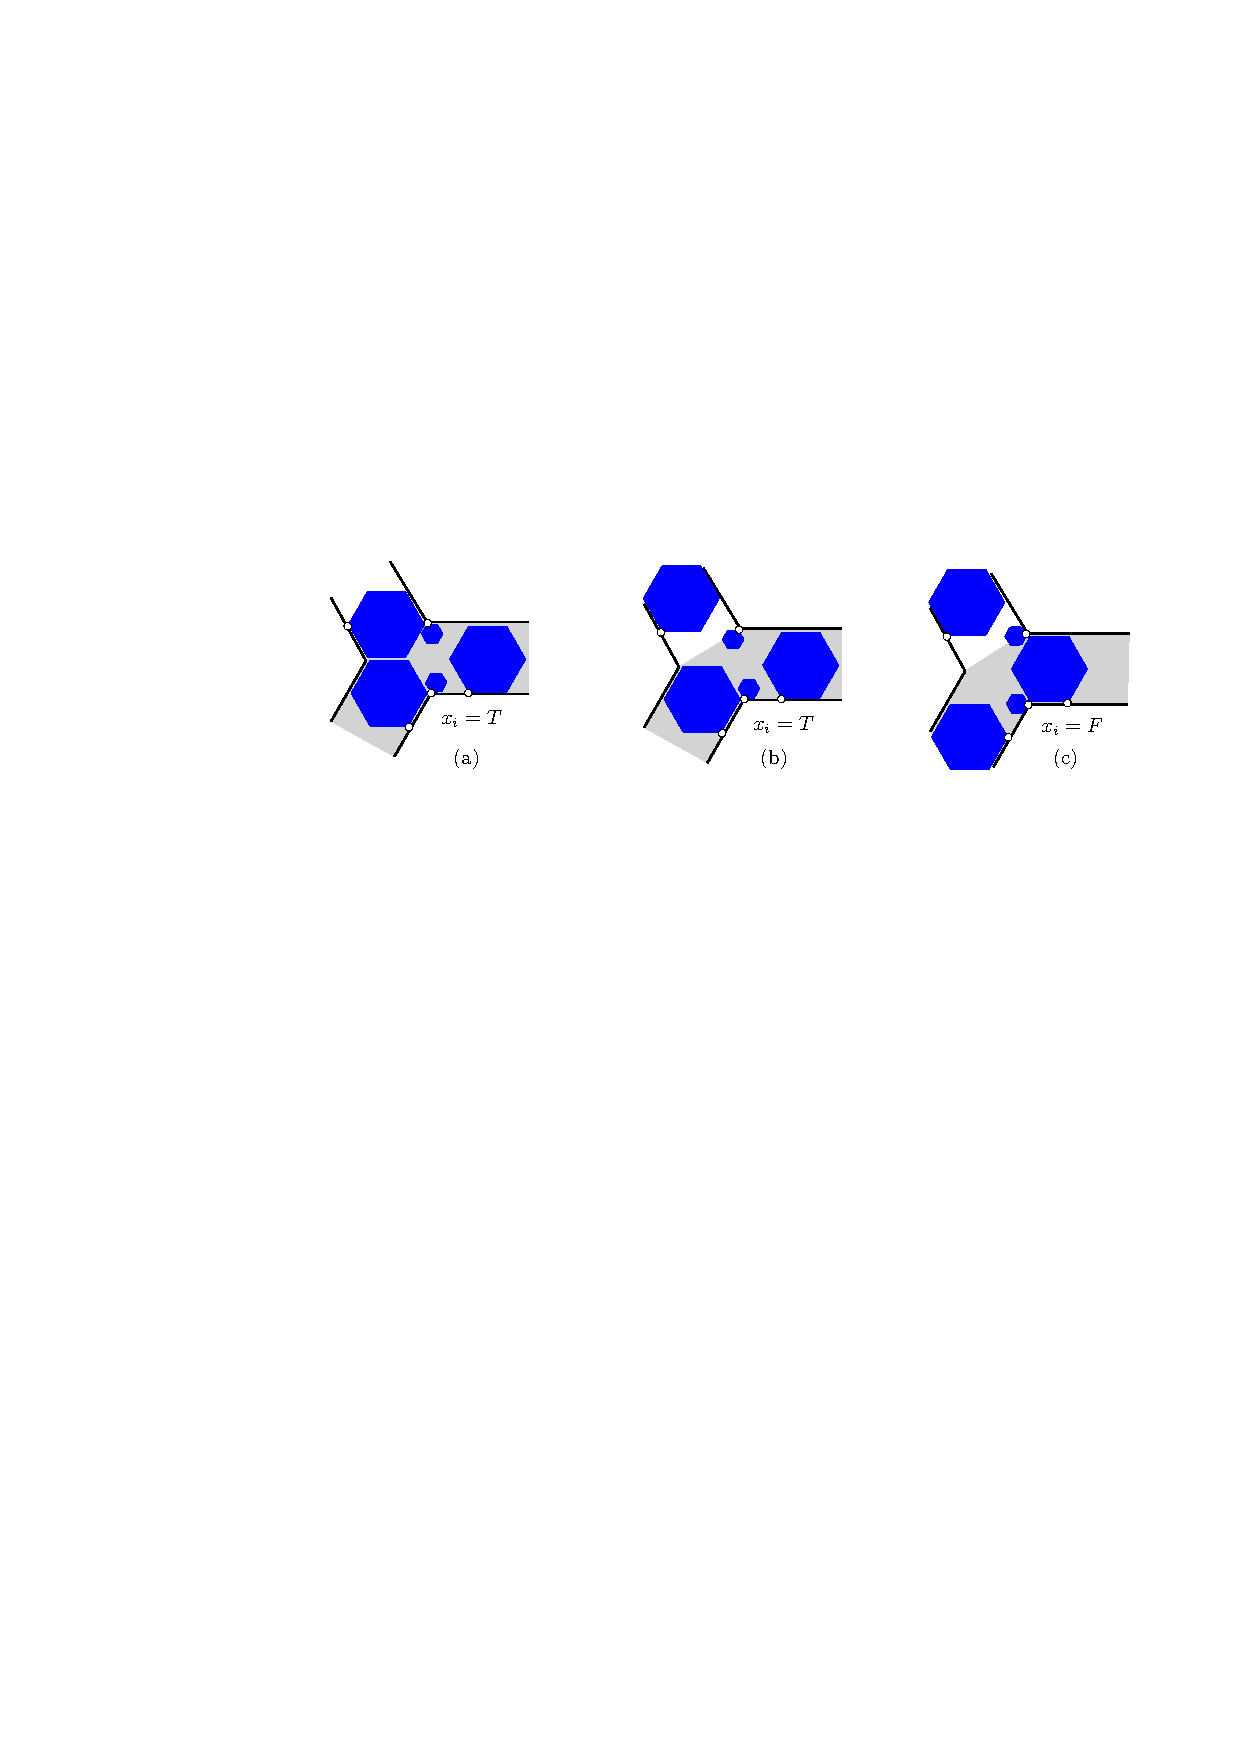
\includegraphics[width=0.7\columnwidth]{graphics/fig-transmitter-hex}
	\captionof{figure}{The common junction of a variable gadget and a transmitter gadget.
(a) When $x_i=T$, a hexagon of the transmitter may enter the junction of the variable gadget.
(b) When $x_i=T$, the transmitter gadget has several possible realizations.
(c) When $x_i=F$, no hexagon from the transmitter enters a junction of the variable gadget.}
	\label{fig:transmitter}
\end{center}
\end{minipage} 

This completes the description of the auxiliary construction.

\section{Functionality of the Auxilary Construction and Gadgets}

For each corridor, there are two junctions adjacent to it; of these two junctions, we denote the junction from which a flag in the corridor enters into as the \textit{active junction} (see Figure \ref{fig:ActiveChannel.pdf}).  
% If the literal $x_i$ (resp., $\overline{x}_i$) appears in $C_j$, then we attach a small hexagon to the corner of this junction such that if $x_i=F$ (resp., $\overline{x}_i=F)$, then the unit hexagon of the transmitter gadget cannot enter this junction. 

\begin{minipage}{\linewidth}
\begin{center}
\includegraphics[width=0.9\columnwidth]{graphics/ActiveChannel.pdf}
\captionof{figure}{The active junction in (a) is the junction on the left and in (b) the active junction is on the right.  The active junction is the junction in which a flag enters from a corridor.}\label{fig:ActiveChannel.pdf}
\end{center}
\end{minipage}

% A variable gadget for vertex $v$ in the associated graph of a P3SAT Boolean formula encompasses at least $2 \cdot \deg (v)$ consecutive obstacle hexagons. 
% The arrangement of the consecutive obstacle hexagons are in staggered fashion about a horizontal line where there are at least $\deg (v)$ obstacle hexagons in the upper portion of the staggering arrangement and at least $\deg (v)$ obstacle hexagons in the lower portion of the staggering arrangement.

Section \ref{sec:auxiliaryConstruction} is a formal description of the auxilary construction and its gadgets.
This subsection covers the underlying assumptions and proofs about the functionality of the auxilary construction.
Throughout this section we assume that the polygonal linkage is realizable, i.e. no two polygons overlap.  
The first observations about the functionality of the auxilary construction are about the flags.  
For $t$ flags in a corridor, the following holds:
\begin{observation}\label{obs:corridor}
\begin{itemize}
\item[(1)] If the leftmost flag is in state R, then all $t$ flags are in state R, and the rightmost flag enters the junction on the right of the corridor.
\item[(2)] Similarly, if the rightmost flag is in state L, then all $t$ flags are in state L, and the leftmost flag enters the junction on the left of the corridor.
\end{itemize}
\end{observation}

Observation~\ref{obs:corridor} and the small hexagons ensure that the state of any flag along the cycle determines the state of all other unit hexagons in the cycle. 
This property defines the binary variable $x_i$: if all flags in the top horizontal corridors are in state R and $x_i=F$, then $x_i=T$ and all hexagons are all in state L.

When a binary variable $x_i = T$, we will say that the variable in state $R$ and that the cycle of small hexagons around the variable gadget are in a ``clockwise direction''.
When a binary variable $x_i = F$, we will say that the variable is in state $L$ and that the cycle of small hexagons around the variable gadget are in a ``counter-clockwise direction''. 

The proof of the Observation \ref{obs:corridor} is similar to the proof of Lemma \ref{lem:logicEngine1} regarding a row in a logic engine having a collision-free configuration.
\begin{proof}
Suppose the leftmost hexagon, $h_1$, is in state $R$ in a corridor.
Denote the $t$ flags in a corridor as $h_1$, $h_2$, $\ldots$, $h_t$ from leftmost to rightmost respectively.
$h_2$ must be in state $R$ otherwise we result in a collision between $h_1$ and $h_2$.
Without losss of generality, $h_i$ and $h_{i+1}$ must be in a state $R$ in order to prevent an adjacent flag collision. 
This implies that rightmost flag $h_t$ must also be in state $R$; this implies that $h_t$ enters the junction that is on the right of the corridor.

Similarly, suppose the rightmost hexagon, $h_t$, is in state $L$ in a corridor.
Denote the $t$ flags in a corridor as $h_1$, $h_2$, $\ldots$, $h_t$ from leftmost to rightmost respectively.
$h_{t-1}$ must be in state $L$ otherwise we result in a collision between $h_t$ and $h_{t-1}$.
Without losss of generality, $h_i$ and $h_{i+1}$ must be in a state $L$ in order to prevent an adjacent flag collision. 
This implies that rightmost flag $h_1$ must also be in state $L$; this implies that $h_1$ enters the junction that is on the left of the corridor.
\end{proof}

% Each junction is a regular triangle, adjacent to three corridors. 
% In some of the junctions, we attach a small hexagon of side length $\frac{1}{3}$ to one or two corners of the junction (see Fig.~\ref{fig:variable}(c) and Fig.~\ref{fig:transmitter}). 
% Importantly, we have the following observation:
\begin{observation}\label{obs:junction}
If a small hexagon is attached to a vertex at a junction between two adjacent corridors, then a flag can enter the junction from at most one of those corridors.
\end{observation}
\begin{proof}
Suppose there is a small hexagon attached to a vertex at a junction between two adjacent corridors.
Suppose it is not that case that a flag can enter the junction from at most one of these adjacent corridors.
Then there are two flags entering the junction, one from each adjacent corridor.
The angular sum of the vertex about the adjacent corridors consists of the obstacle hexagon, both flags, and the small unit hexagon.
Each angle of each hexagon is $\frac{2 \pi}{3}$ radians, totalling to an angular sum of $\frac{8 \pi}{3} > 2 \pi$.
This is a contradiction with the total angular sum of a vertex on the plane to be $2 \pi$.
\end{proof}

The flags of the auxilary construction help communicate the boolean value of a variable gadget to the rest of the auxilary construction.
This communication property of the flags in a corridor is analagous to the flags in a row of a logic engine.

Observations \ref{obs:corridor} and \ref{obs:junction} ensure that the state of any unit hexagon along the cycle determines the state of all other unit hexagons in the cycle. 
This property defines the binary variable $x_i$: If $x_i=T$, then all unit hexagons in the top horizontal corridors are in state R; and if $x_i=F$, they are all in state L.

For a variable gadget $x_i$, we distinguish the upper half and lower half of the gadget in the variable cycle.
Then we have the following lemma:
\begin{lem}\label{lem:aux-2}
If variable $x_i = T$, then all flags in the upper half of the variable gadget are in state $R$ and all flags in the lower half of the variable are in state $L$; if variable $x_i = L$, then all flags in the upper half of the variable gadget are in state $L$ and all flags in the lower half of the variable gadget are in state $R$.    
\end{lem}
This lemma servers to show that the truth or falsity of a variable is consistent throughout the gadget.
\begin{proof}
Suppose we have two adjacent corridors $k_i$ and $k_{i+1}$ sharing junction $J_i$ and without loss of generality, $k_i$ is the left most corridor.
Observation \ref{obs:junction} implies that there can only be one hexagon entering $J_i$ from either $k_i$ or $k_{i+1}$. If the hexagon that enters $J_i$ is from corridor $k_i$, then this hexagon has state $R$ and all flags in corridor $k_i$ are in state $R$ by Observation \ref{obs:corridor}. 
Since the nearest flag of corridor $k_{i+1}$ cannot enter the junction $J_i$, it must also have state $R$.  
All flags in corridor $k_{i+1}$ are in state $R$ by Observation \ref{obs:corridor}. 

The argument is similar if the hexagon entering $J_i$ is from corridor $k_{i+1}$ and all flags in both corridors $k_i$ and $k_{i+1}$ have state $L$.

Because variable gadgets form a simple cycle of corridors and junctions $\lr{k_1, J_1, k_2, J_2, \dots, k_n, J_n}$ and the argument above, all flags about a variable gadget have the same state.
\end{proof}

Suppose there is an edge $\left\lbrace x_i, C_j \right\rbrace$ in the graph $A(\Phi)$:
\begin{lem}\label{lem:aux-3}
If $x_i = T$ and its negated literal is in $C_j$, then a flag enters into the clause gadget of $C_j$, otherwise it need not enter; if $x_i = F$ and its non-negated literal is in $C_j$, then a flag enters into the clause gadget of $C_j$, otherwise it need not enter.
\end{lem}
\begin{proof}
The transmitter gadget for each literal is placed on an active junction of the variable gadget. 
This junction is ``activated'' by the variable gadget.  
By Observation \ref{obs:junction}, the flag nearest of the transmitter gadget to the variable gadget does not enter the transmitter-variable junction.
By Observation \ref{obs:corridor} and the state of the flag nearest of the transmitter gadget to the variable gadget implies that the flags in that transmitter corridor activate the junction opposite the transmitter-variable junction.
The subsequent flags in the transmitter gadget corridors have the same state of the flag in the transmitter gadget nearest of the transmitter-variable junction by Observations \ref{obs:corridor} and \ref{obs:junction}.
This activation process continues up to the clause junction and the flag in the transmitter gadget nearest the clause junction enters the clause junction.
\end{proof}

\begin{lem}\label{lem:aux-1}
Hexagons in a clause junction have a non-overlapping placement if and only if at least one of the three literals is true.
\end{lem}
\begin{proof}
Suppose we have a hexagons in a clause junction that have a non-overlapping placement.
To show that there is at least one of the three literals is true,  we do a proof by contradiction.
Suppose all literals of the clause are false.
If all literals of the clause are false, then all flags in each transmitter gadget nearest their clause junction enters the clause junction, as shown in Figure \ref{fig:clause}(c) which show the small hexagon overlapping flags in the clause junction, a contradiction with hexagons in the clause junction have a non-overlapping placement.

If at least one of the three literals is true, then by Lemma \ref{lem:aux-3}, this literal's flag need not enter the transmitter-variable junction.
There allows for the small hexagon in the clause junction to move into the area where this literal's flag could enter the junction and thus allow non-overlapping placement of hexagons in the junction.
\end{proof}



\begin{lem}\label{lem:aux-A}
For every instance $\Phi$ of P3SAT, the above polygonal linkage with flexible and obstacle polygons has the following properties: (1) it has polynomial size; (2) its hinge graph is a forest;
(3) it admits a realization such that the obstacle polygons remain fixed if and only if $\Phi$ is satisfiable.
\end{lem}
\begin{proof}

We can bound the number of obstacle hexagons to represent a variable gadget by $2 D$, where $D = \lr{ \max_{v \in V} \deg (v)}$.  
The number of clause junctions is $n$.
To give an upper bound on the number of flags in the auxiliary construction, we have to account for the flags in the transmitter gadgets, the extra hexagons found in junctions, and the flags around the variable gadgets.

Recall that that the number of flags in a corridor are $ t = 2N(m,n)^3 + 1 $ where $N(m,n)$ is a polynomial. 
Recall that the drawing of $A(\Phi)$ have edges drawn in vertically and horizontally and can join at some ``elbow''.  
The distance can be measured in the $\ell_1$ norm.
Similarly in the honeycomb construction, the flexable hexagons zig-zig vertically and horizontally through out honeycomb.  
The number of corridors about an obstacle hexagon is $6$.
A generous upper bound on the number of flags in a transmitter gadget, is $6 \cdot t \cdot \ell_1\lr{v_i,C_j}$, assuming each obstacle hexagon is of unit height.

The number of junctions in the auxiliary construction is the number of junctions to form all variable gadgets, transmitter gadgets, and clause gadgets. 
We know there are at most $2 \cdot D$ obstacle hexagons to form each variable gadget and $6$ junctions for each obstacle hexagon.  
Therefore an upper bound for the number of flags around variable gadgets is $m \cdot 6 \cdot t \cdot 2 \cdot D$.
An upper bound for the number of junctions in a transmitter gadget is $6 \ell_1 \lr{v_i, C_j}$.  
Thus, an upper bound of all junctions in all transmitter gadgets is $$6 \cdot \sum_{\left\lbrace v_i, C_j \right\rbrace \in E} \ell_1 \lr{v_i, C_j}.$$
It is further upper bounded by  $J_d$:
$$6 \cdot \sum_{\left\lbrace v_i, C_j \right\rbrace \in E} \ell_1 \lr{v_i, C_j} \leq 12 (m+n) J_d(n,m)$$
where $2 (m+n)$ is the maximum number of edges in a planar bipartite graph with $(m+n)$ vertices.  
An upper bound on the total number of flags is
$$m \cdot 6 \cdot t \cdot 2 \cdot D + 12 (m+n) J_d(n,m).$$

\noindent (2) Recall that a forest is a disjoint union of trees. 
By construction, each flag is hinged to exactly one obstacle hexagon.  
There are no hinges between obstacle hexagons.
Consequently, each component of the hinge graph is a star, where the center corresponds to an obstacle hexagon and the leafs corresponds to the flexable hexagons attached to it.

\noindent (3) The final statement is to show an if and only if statement: it admits a realization such that the obstacle polygons remain fixed if and only if $\Phi$ is satisfiable.

Suppose $\Phi$ is satisfiable.  % and has $m$ variables $x_1$ through $x_m$ and $n$ clauses $C_1$ through $C_n$.
Each variable has a boolean value and we can encode the corresponding auxilary construction accordingly.  
For each variable, we encode the boolean value by the state of the flags surrounding the variable gadget to $R$ or $L$.  
Lemma \ref{lem:aux-2} shows that the corridors and junctions around the variable gadget are realizable.
Lemma \ref{lem:aux-3} also show that for each transmitter gadget, every corridor and junction are also realizable. 
Lemma \ref{lem:aux-1} shows that there is at least one hexagon in the clause junction and that the clause is realizable.
Thus all parts of the auxilary construction realizable and thus we have a realization.

Suppose the construction admits a realization such that the obstacle polygons remain fixed.
Each variable gadget's flags are configured to state $L$ or $R$. 
The variable's corresponding state correspond to the variable's truth value, i.e. $R$ for true and $L$ for false.
Using Lemma \ref{lem:aux-2}, the boolean state of the variable gadget is transmitted to all transmitter gadgets associated to it.
Each clause is realizable and so for every clause, there exists one true literal in the clause corresponding to a variable by Lemma \ref{lem:aux-1}. 
If every clause has some true literal, then the corresponding 3-CNF boolean formula is satisfiable.
\end{proof}
